\chapter{Filtering} \label{ch7}
It is wanted to reduces noise on the music signal that is to be processed by the application hence this chapter introduces the basic filter theory necessary for the system. Basic theory concerning mathematically ideal filters is described, followed by techniques for design of practical non ideal filters. This chapter is inspired by \cite{DTSP, ch. 5,7} and \cite{FSP, sec. 3.4.4}\\
Note that filters concerned in the project are only digital filters, meaning the filter is a algorithm to be executed on a computer. An analog filter is in contrast constructed by physical component. Both types relay on the input/output relation that are to be mathematical represented.     
\section{Basic principles} \label{sec:basic_filter}
A digital filter is characterised as an LTI system, previously defined by equation \eqref{eq:LTI_diff_equation_finite}. As described the system is completely characterized by its corresponding impulse response $h[n]$. In terms of the LTI system as a filter the output $y[n]$ is the part of the signal that comes through the filter. \\
$y[n]$ was previous defined by \eqref{def:convolution} as the convolution sum of input signal and impulse response of the system
\begin{align}
y[n] = x[n]*h[n] = \sum_{k=-\infty}^{\infty} x[k]h[n-k].
\end{align}    
The frequency response of the system is given by the Fourier transform of the impulse response - analogue to definition \ref{def:Fourier_trans} for a discrete sequence - as
\begin{align}\label{eq:freq_res}
H(\omega)=\sum_{k=-\infty}^{\infty}h[k]e^{-j\omega k}.
\end{align}
It is known from the definition that $H(\omega)$ can be expressed as
\begin{align}
H(\omega)=|H(\omega)|e^{j\measuredangle H(\omega)},
\end{align}  
where $|H(\omega)|$ and $e^{j\measuredangle H(\omega)}$ are the \textit{amplitude} and \textit{phase} response of the filter respectively, both real valued and $2\pi$-periodic.\\
If $H(\omega)$ is real it is said to have \textit{zero phase}, which is equivalent to the phase response only taking values that are integer multiples of $\pi$, resulting in a straight phase with zero slope. Further if $H(\omega)$ can be written in the form 
\begin{align}\label{eq:lin_pha}
H(\omega)=A(\omega)e^{j(-\alpha\omega + j\beta)} ,
\end{align}
where $\alpha$ and $\beta$ are constants and $A(\omega)$ is real, the filter is said to have \textit{general linear phase}. That is because the phase response consists of constant terms added to the linear function making a straight line with slope $\alpha$ except from the discontinuities resulting from jumps of $2\pi$ caused by the $2\pi$-periodicity. \\
A generalized linear phase response is characterized by a constant \textit{group delay} $\tau(\omega)$:
\begin{align}
\tau(\omega)=-\frac{d}{d\omega}\left\{ \measuredangle H(\text{e}^{j\omega} \right\} = \alpha.
\end{align}
The phase response is an expression of how each of the signal components are delayed though the system, where linear phase indicates an equal delay for all components of the signal. To guarantee a constant group delay, $\alpha$, $\beta$ and $h[n]$ has to fulfil the following condition, for all $\omega$ \cite{DTSP, page 341}
\begin{align}\label{eq:cons_gro}
\sum_{n=-\infty}^{\infty}h[n]\sin\left(\omega \left(n-\alpha \right) + \beta \right) = 0.
\end{align}

\subsection{Ideal filters} \label{sec:ideal_filt}
When designing filters it is ideal to have constant amplitude and zero phase corresponding to the frequency response. \\ For an ideal selective frequency filter the amplitude response will be constant unity for the frequencies that are wanted to pass the filter referred to as the \textit{bandpass} and zero for all other frequencies referred to as \textit{bandstop}. An example is an ideal lowpass filter with frequency response 
\begin{align}\label{eq:low}
H_{lp}(\omega)=
\left\{ \begin{matrix}
1, &\ \left| \omega \right|< \omega_c \\
0, &\ \omega_c < \left| \omega \right| \leq \pi
\end{matrix}\right.,
\end{align}     
where $H_{lp}(\omega)$ is $2\pi$ periodic. $\omega_c$ is referred to as the \textit{cutoff frequency}. The lowpass filter selects the frequencies lower than the cutoff frequency and reject the higher frequency components of the input signal. By \eqref{eq:low} it is seen that the lowpass filter is real valued hence has zero phase as expected. \\
The corresponding impulse response are determined by the inverse Fourier transform on the passband interval - analogue to definition \ref{def:InverseFourier_trans} for a discrete sequence.
\begin{align}\label{eq:low_im}
h_{lp}[n]= \frac{1}{2\pi}\int_{-\pi}^{\pi}\text{e}^{j\omega n} d\omega =\frac{1}{2\pi}\int_{-\omega_c}^{\omega_c}\text{e}^{j\omega n} d\omega = \frac{1}{2\pi j n}\left[\text{e}^{j\omega n} \right]_{-\omega_c}^{\omega_c} = \frac{\sin \omega_c n}{\pi n }, \ \  -\infty < n < \infty.
\end{align} 
Note that the first equality is true because by \eqref{eq:low} the integral is zero outside the interval $[-\omega_c, \omega_c]$. \eqref{eq:low} is only true for $n \neq 0$ and $h_{lp}[0]$ must be defined separately. For this l'Hôspitals rule $\lim \frac{f(x)}{g(x)}=\lim \frac{f'(x)}{g'(x)}$ is used. Thus
\begin{align}
h_{lp}[0]=& \frac{1}{\pi} \left( \cos\left( \omega_{c} n \right)\omega_{c}\right)
= \frac{1}{\pi}\left( \omega_{c} \right).
\end{align}

By \eqref{eq:low_im} the impulse response is non-zero for all $n<0$ thus the filter is non-casual according to definition \ref{def:causal_system}.\\
Amplitude- and impulse response of the ideal lowpass filter are illustrated on figure \ref{fig:ideal_low}
\begin{figure}[H]
\begin{subfigure}[b]{0.50\textwidth}
        \centering
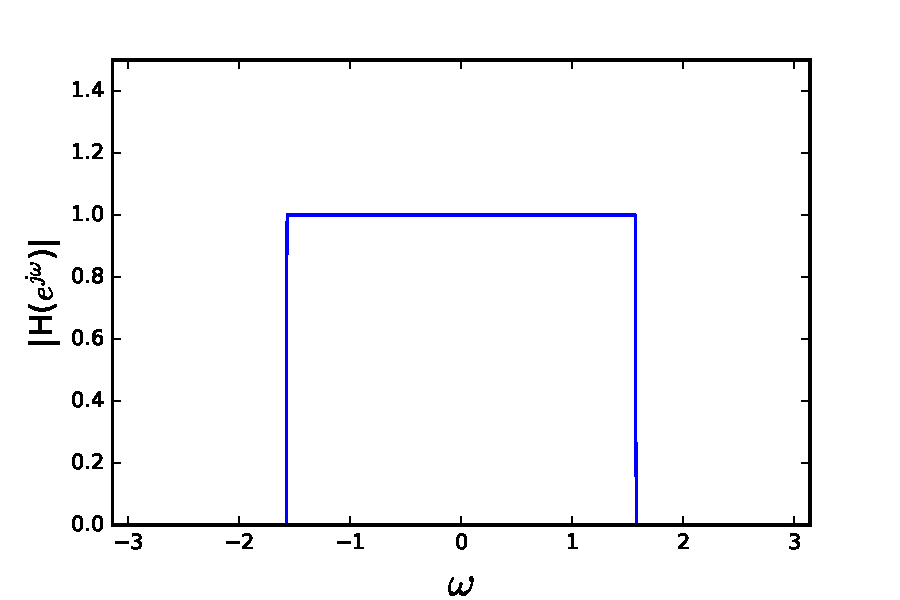
\includegraphics[scale=0.45]{figures/filter_teori/ideal_low2.pdf}
\caption{}
\end{subfigure}
\begin{subfigure}[b]{0.50\textwidth}
        \centering  
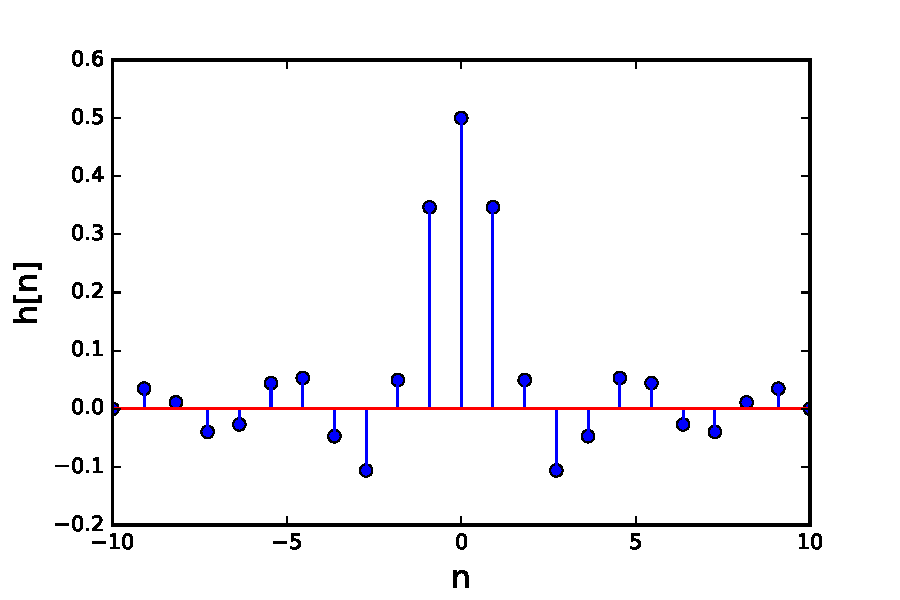
\includegraphics[scale=0.45]{figures/filter_teori/ideal_low1.pdf}
\caption{}
 \end{subfigure}
\caption{ (a) Amplitude response of ideal lowpass filter with $\omega_c = \frac{\pi}{2}$ (b) corresponding impulse response}
\label{fig:ideal_low}
\end{figure}


Analogues of ideal highpass or bandpass filter can be defined, as illustrated on figure \ref{fig:ideal}.\\ 

\begin{figure}[H]
\begin{subfigure}[b]{0.50\textwidth}
        \centering
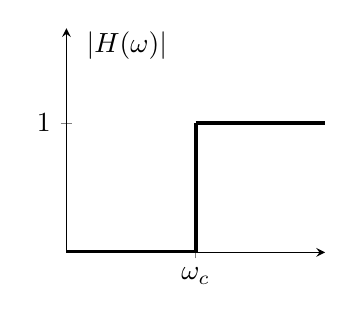
\begin{tikzpicture}[scale=1]
\begin{axis}[
scale=0.5,
unit vector ratio*=1 1 1,
axis lines = middle,
xtick={1.5},
xticklabels={$\omega_c$},
ytick={1.5},
yticklabels={$1$},
xmin=0,
xmax=3,
ymin=0,
ymax=2.6]
\node at (axis cs:0.7,2.4) {$|H(\omega)|$};
\draw[line width=0.6mm](axis cs:0,0)--(axis cs:1.5,0);
\draw[line width=0.5mm](axis cs:1.5,1.5)--(axis cs:3,1.5);
\draw[line width=0.5mm](axis cs:1.5,1.5)--(axis cs:1.5,0);
\end{axis}
\end{tikzpicture}

\caption{}
    \end{subfigure}
 \begin{subfigure}[b]{0.50\textwidth}
        \centering  
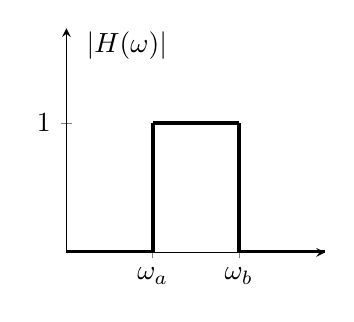
\begin{tikzpicture}[scale=1]
\begin{axis}[
scale=0.5,
unit vector ratio*=1 1 1,
axis lines = middle,
xtick={1,2},
xticklabels={$\omega_a$,$\omega_b$},
ytick={1.5},
yticklabels={$1$},
xmin=0,
xmax=3,
ymin=0,
ymax=2.6]
\node at (axis cs:0.7,2.4) {$|H(\omega)|$};
\draw[line width=0.5mm](axis cs:1,1.5)--(axis cs:1,0);
\draw[line width=0.5mm](axis cs:1,1.5)--(axis cs:2,1.5);
\draw[line width=0.5mm](axis cs:2,1.5)--(axis cs:2,0);
\draw[line width=0.5mm](axis cs:1,0)--(axis cs:0,0);
\draw[line width=0.5mm](axis cs:2,0)--(axis cs:3,0);
\end{axis}
\end{tikzpicture}
\caption{}
    \end{subfigure}
\caption{Amplitude response of ideal (a) highpass filter (B) bandpass filter}
\label{fig:ideal}
\end{figure}
As stated in section \ref{sec:LTI} a non-causal LTI system is not realizable. Furthermore  zero phase is not possible for a causal system.
Thus an approximation of an ideal filter can be computed by a casual system with general linear phase.    

\section{FIR and IIR filter} 
Two classes of filter are essential to identify.
For all ideal filters discussed in the previous section the impulse response is defined for $-\infty < n < \infty$. Such a filter is specified as an \textit{infinite impulse response (IIR)} filter. In the case of the impulse response being zero outside a finite interval the filter is referred to as a \textit{finite impulse response (FIR)} filter. 
\subsection{Type 1 FIR filter}
As described causal systems with generalized linear phase is a possible approximation of the ideal filter. This is to be guaranteed by using specific types of FIR filters.\\
A causal system with generalized linear phase has to fulfil the following relation, cf. section \ref{sec:basic_filter}:
\begin{align}
\sum_{n=0}^{\infty}h[n]\sin\left(\omega \left(n-\alpha \right) + \beta \right) = 0
\end{align}
For a FIR filter to satisfy this relation the following set of conditions has to be fulfilled \cite{DTSP, p.342}:
\begin{align} \label{eq:FIR_con}
&\beta = \left\{ \begin{matrix} 
\pi  \\
0 
\end{matrix}\right. \nonumber  \\ 
&2\alpha = M = \text{an integer} \\ 
&h[n]=h[M-n] \ \text{or} \ h[n]=-h[M-n]. \nonumber  
\end{align} 
This implies that $h[n]$ is either symmetric or anti symmetric and that $\alpha = \frac{M}{2}$ becomes the symmetry point. \\
From these conditions four different types of FIR filter with generalized linear phase are defined \cite{DTSP, page 343}, only the \textit{type 1 FIR filter} will be elaborated here.
A type 1 FIR filter is characterised by having a symmetric impulse response and $M$ being an even integer. By applying the symmetry condition to the definition of the Fourier transform $H(\omega)$ is defined as \cite{page 343,DTSP}   
\begin{align}\label{eq:type1}
H(\omega)=\text{e}^{-j\omega \frac{M}{2}} \sum_{k=0}^{\frac{M}{2}} a[k]\cos \omega k,
\end{align}
where 
\begin{align}
a[k]= \left\{ \begin{matrix}
2h\left[ \frac{M}{2} - k \right], \ \ &\ k=1,2,... , \frac{M}{2}.   \\
h[\frac{M}{2}], \ \ &\ k = 0  
\end{matrix}\right.
\end{align}
By this \eqref{eq:type1} has the form of \eqref{eq:lin_pha} where $A(\omega)= \sum_{k=0}^{\frac{M}{2}} a[k]\cos \omega k$ is a real function of $\omega$ and $\beta$ equals either 0 or $\pi$. Hence a constant group delay is achieved.








   
 


 




\section{Filter design}
In this section the process of designing digital filter are described. There will be a distinguished between techniques for IIR and FIR filters..\\
As described ideal filters are not computable hence the process of designing a filter is based on approximation of the frequency response made by computable polynomials.  


\subsection{IIR filter}
One common way of designing an IIR-filter is to design the discrete-time filter from a corresponding continuous-time system. The idea follows four main steps. 
\begin{itemize}
\item[1.] Specify the properties desired for the filter.
\item[2.] Hereby compute a "prototype" by a continuous-time system $H_c(j\Omega)$ that approximates the given properties.
\item[3.] Transform the "prototype" into the discrete-time filter $H(e^{j\omega})$ by...
\item[4.] Implementation of the filter. 
\end{itemize}
The properties of a system are specified on behave of the desired application, considering what frequencies are to pass the filter ideally. Further it is important to specify how much the filter are allowed to vary from the ideal properties, from which it will vary. \\
Properties for an approximation to a lowpass filter could be defined by bounding the magnitude within $\pm \ \delta_1$ of unity in a limited frequency band $0 \leq \Omega \leq \Omega_p $ and less than $\delta_2$ in the frequency band $\Omega_s \leq \Omega$\trine{beskrivelse af convertering af spec. er udkommenteret}. 
The tolerance scheme pleasing the continuous-time filter is illustrated on figure \ref{fig:scheme}\\ 
The transition off nonzero width between the cutoff frequency of passband and stopband is necessary in order for the system to be realizable.

\begin{figure}[H]
\centering
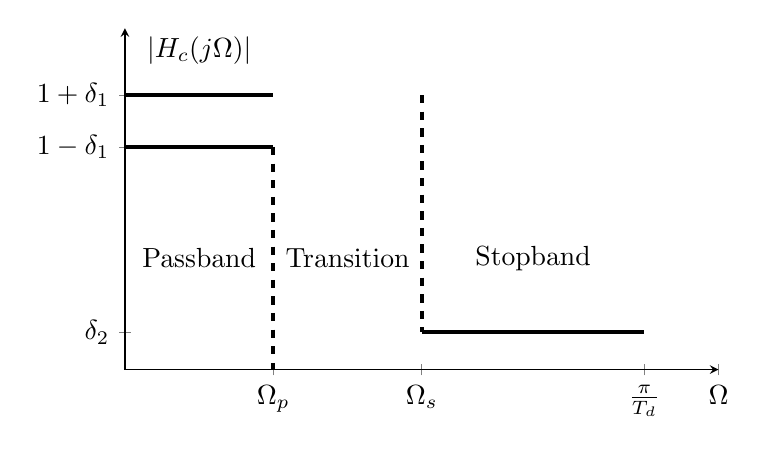
\begin{tikzpicture}[scale=1]
\begin{axis}[
scale=1.1,
unit vector ratio*=1 1 1,
axis lines = middle,
xtick={0,2,4,7,8},
xticklabels={$0$,$\Omega_p$,$\Omega_s$,$\frac{\pi}{T_d}$,$\Omega$},
ytick={0.5,3,3.7},
yticklabels={$\delta_2$,$1-\delta_1$,$1+\delta_1$},
xmin=0,
xmax=8,
ymin=0,
ymax=4.6]
\node at (axis cs:1,4.3) {$|H_c(j\Omega)|$};
\draw[line width=0.5mm](axis cs:0,3.7)--(axis cs:2,3.7);
\draw[line width=0.5mm](axis cs:0,3)--(axis cs:2,3);
\draw[line width=0.5mm, dashed](axis cs:2,3)--(axis cs:2,0);
\draw[line width=0.5mm, dashed](axis cs:4,3.7)--(axis cs:4,0.5);
\draw[line width=0.5mm](axis cs:4,0.5)--(axis cs:7,0.5);
\node at (axis cs:1,1.5) {Passband};
\node at (axis cs:3,1.5) {Transition};
\node at (axis cs:5.5,1.5) {Stopband};
\end{axis}
\end{tikzpicture}
\caption{Specification of frequency response}
\label{fig:scheme}
\end{figure}

Methods for defining a continuous-time system that fits the specification are establish as known continuous-time filter designs. The \textit{Butterworth filter} which is a lowpass filter approximation will now be described along with the Bbiliniare transformation.\\
For a Butterworth filter the squared magnitude are defined as follows.
\begin{align}\label{eq:butter}
|H_c(j\Omega)|^2=\frac{1}{1+\left( \frac{j\Omega}{j\Omega_c}\right)^{2N}}
\end{align} 
Further the filter is characterised by the following three properties.
\begin{align}
1.& \ \ \ |H_c(j\Omega)|^2 = 1 \  \ \left|\begin{matrix}
\\ 
\Omega=0
\end{matrix}\right. , \textit{ for all }N. \\
2.& \ \ \ |H_c(j\Omega)|^2 = \frac{1}{2} \  \ \left|\begin{matrix}
\\ 
\Omega=\Omega_c
\end{matrix}\right. , \textit{ for all }N. \\
3.& \ \ \ \textit{Magnitude response is monotonic in pass- and stopband.}
\end{align}
As the order $N$ of the filter increases the characteristics become sharper and the filter approximates the ideal lowpass filter. This is illustrated on figure \ref{fig:butter}. By\eqref{eq:butter} it is possible to compute the order necessary for the system to fulfil the specifications.            
\begin{figure}[H]
    \centering
    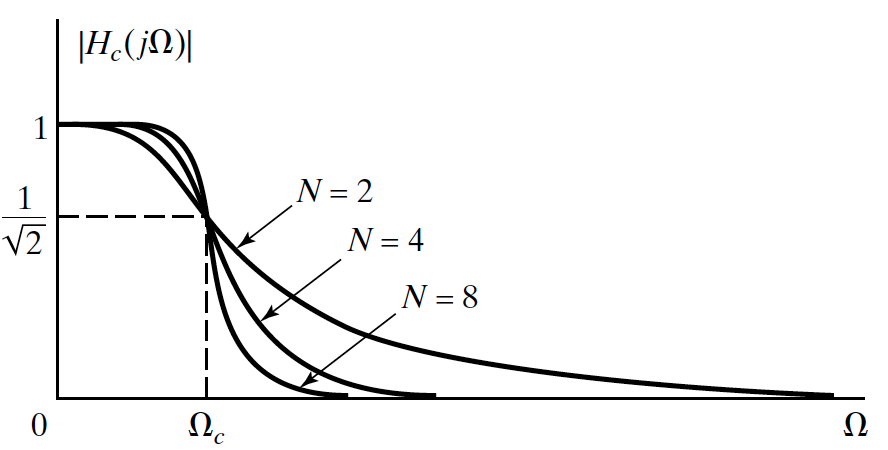
\includegraphics[width = 0.6\textwidth]{figures/butterworth.png}
    \caption{Magnitude of Butterworth filter depending on order $N$ }
    \label{fig:butter}
\end{figure} 
In order to obtain causality and stability in the system representation in the $s$-domain is wanted. By substituting $s=j\Omega$ the following relation is true.
\begin{align}
|H_c(j\Omega)|^2 = H_c(s)H_c(-s)= \frac{1}{1+\left( \frac{s}{j\Omega_c}\right)^{2N}}
\end{align} 
By letting the denominator in \eqref{eq:butter} equal to zero it is possible to determine the poles $s_k$ of the system as 
\begin{align}
s_k = (-1)^{\frac{1}{2N}}\left(j\Omega_c\right)=\Omega_c\text{e}^{\left(\frac{j\pi}{2N}\right)\left(2k+N-1\right)}, \ \ k=0,1,\ ... \ , 2N-1 
\end{align}   
The poles will placed equally along the circle of radius $\Omega_c$ as illustrated on figure \ref{??}. By only considering the poles in the left half plane $H_c(s)$ can be construed as a stable system. 
\begin{align}
H_c(s)=\frac{1}{\prod_{k=1}^{N}(s-s_k)}
\end{align}    
When the continuous-time filter $H_c(s)$ is defined the next step is the transformation from continuous-time to discrete-time. The bilinear transformation is a method that allows a direct transformation between the s- and z-domain. The principal of the transformation is that the imaginary axis $j\Omega$ of the s-plane is mapped onto the z-plane as the unitcircle. The bilinear transformation is defined by 
\begin{align}
s=\frac{2}{T_d}\left(\frac{1-z^{-1}}{1+z^{-1}}\right) 
\end{align}
such that 
\begin{align}
H_c\left[\frac{2}{T_d}\left(\frac{1-z^{-1}}{1+z^{-1}}\right)\right]=H_c(z), 
\end{align}  
Because $-\infty \leq \Omega \leq \infty $ is mapped to $-\pi \leq \omega \leq \pi$ the transformation most be non linear which involves some frequency distortion. By this the method is restricted to situations where this is acceptable or can be compensated. Compensation can be done by the concept of pre wrapping, that consider the relation 
\begin{align}
\Omega_{c_{new}}=\frac{2}{T_d}\tan\frac{\omega_c}{2}
\end{align}
hereby it is possible to determine a new $\Omega_c$ to the continuous-time filter, in order to ensure the discrete $\omega_c$ to fit the specification.\\
An important property of the bilinear transformation is that stability is preserved if the continuous-time filter i stable. \\
... \\
Advantages of IIR filter:
The process of designing a IIR filter is rather simple when the desired properties fits an establish design method such as a Butterworth filter. The required order of the filter is computable and the transformation to the discrete-time domain is to be done straight forward. Further, considering the implementation, this leads to non iterative algorithms. \\
Though by this method the magnitude response is the only parameter to be specified. Meaning that specific requirements for e.g. phase response or group delay are not quarantined to be fulfilled by this kind of IIR filter.

%
%These properties are to be converted into specifications of the discrete-time filter by expressing the frequency in normalised radian frequency by the relation $\omega=\Omega T_d$ where $T_d$ is the sampling rate. Thus the impulse response is specified over one period as 
%\begin{align}
%H_c(j\Omega)=H(e^{j\omega}), \ \ |\omega|<\pi
%\end{align}    
%
%The desired gain of the magnitude is often expressed in dB, where $20\log(1)=0[\text{dB}]$ \trine{is gain of magnitude a thing?} \\
 

\subsection{FIR filter}
Design of FIR filters are in contrast to IIR filters based on approximating the desired discrete-time frequency response directly. By this method it is possible to guarantee a general linear phase of the system. The window method..   

\subsubsection{The Window method}
The window method is considered a simple method for designing FIR filters. The method takes off from the desired frequency response $H_d$ whereby the desired impulse response is obtained by the inverse Fourier transformation of frequency response
\begin{align}
h_d[n]=\frac{1}{2\pi}\int_{-\pi}^{\pi} H_d(\text{e}^{j\omega})\text{e}^{j\omega} d\omega
\end{align}
The idealized frequency response usually results in impulse responses of infinite length and discontinuities at the boundaries between pass- and stopband. To compute a finite casual system as a FIR filter on behave of the desired impulse response the realisable impulse response of the FIR filter is determined as a product of the idealised impulse response $h_d[n]$ and a finite duration \textit{window} $w[n]$ 
\begin{align}
h[n]=h_d[n]w[n], \ \ w[n] =
\left\{ \begin{matrix}
f[n], &\ 0 \leq n \leq M \\
0, &\ Otherwise
\end{matrix}\right.
\end{align}       
By this truncation the impulse response of a finite filter of order $M$ is determined such that
\begin{align}
h[n]= 
\left\{ \begin{matrix}
h_d[n], &\ 0 \leq n \leq M \\
0, &\ Otherwise
\end{matrix}\right.
\end{align}
By Fourier transformation the frequency response of the filter becomes the periodic convolution 
\begin{align}
H(e^{j\omega})=\frac{1}{2\pi}\int_{-\pi}^{\pi} X(e^{j\theta})W(e^{j(\omega-\theta})d\theta
\end{align} 
This is illustrated by an example of the simple \textit{rectangular window} defined as 
\begin{align}
w[n] =
\left\{ \begin{matrix}
1, &\ 0 \leq n \leq M \\
0, &\ Otherwise
\end{matrix}\right.
\end{align}
which by Fourier transformation gives 
\begin{align}
W \left(\text{e}^{j\omega}\right)=\sum_{n=0}^{M} \text{e}^{j\omega n} = \frac{1- \text{e}^{-j\omega(M+1)}}{1- \text{e}^{-j\omega}} = \text{e}^{-j\omega \frac{M}{2}} \frac{ \sin \left( \frac{\omega \left( M+1 \right)}{2} \right)}{\sin \left( \frac{\omega}{2} \right)} 
\end{align}

Figure \ref{fig:FIR1} illustrates the convolution process referred to as windowing\trine{lav selv præcis figur}. note that ripples appear in both pass and stopband. 
\begin{figure}[H]
    \centering
    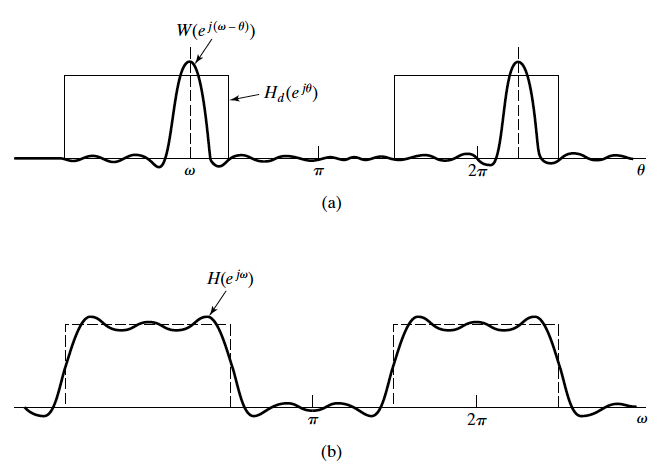
\includegraphics[scale=0.4]{figures/FIR1.png}
    \caption{a) Frequency response $H(e^{j\omega})$ and Fourier transformation of window $W(e^{j\omega})$ b) Approximation of $H(e^{j\omega})$ resulting from windowing the desired impulse response.}
    \label{fig:FIR1}
\end{figure}  
The aim is to approximate the desired frequency response as good as possible. For $w[n]=1 \ \forall \ n$, $W(e^{j\omega})$ becomes a periodic impulse which implies $H(e^{j\omega})=H_d(e^{j\omega})$ though the needed truncations is not performed. The impulse train is best approximated by letting the main lobe of $W(\text{e}^{j\omega})$ be as narrow as possible and the side lobes as small as possible. This corresponds respectively to minimizing the width of the transitband and the ripples in pass and stop band, though it is not possible to achive both at ones.\\
By increasing M the with of the main-lope is decreased, but the peak amplitude of the side-lopes also increases which results in ripples. this indicates a trade-off between main width of main-lope and amplitude of side-lopes. \\
Figure \ref{?} illustrates main and side lope by a plot of the magnitude response corresponding to the rectangular window\trine{indsæt figur}.

\subsubsection{Window types}
The rectangular window is one out of many windows, that have different properties. The oscillations in the frequency response is a result of Gibbs phenomenon. According to converges of Fourier series\trine{uddybes her?} this can be improved by convolving the desired frequency response with a less abrupt window. So by narrowing each end of the rectangle smoothly towards zero, the amplitude peak of the side-lopes are remarkable decreased. Though this will still result in a wider main-lope. \\
In table \ref{tab:window} some commonly used windows are defined, further the window and the corresponding Fourier transformation are illustrated on figure \ref{?}

\begin{table}[H]
\centering
\caption{Definition of different types of windows}
\label{tab:window}
\begin{tabular}{l|l} \hline
Rectangular & $w[n] =
\left\{ \begin{matrix}
1, &\ 0 \leq n \leq M \\
0, &\ Otherwise
\end{matrix}\right. $ \\ \hline
Bartlett    & $w[n] =
\left\{ \begin{matrix}
\frac{2n}{M}, &\ 0 \leq n \leq \frac{M}{2} \\
\frac{2-2n}{M}, &\ \frac{M}{2} \leq n \leq M \\
0, &\ Otherwise
\end{matrix}\right.$ \\ \hline
Hanning     & $w[n] =
\left\{ \begin{matrix}
0.5-0.5 \cos(\frac{2\pi n}{M}), &\ 0 \leq n \leq M \\
0, &\ Otherwise
\end{matrix}\right. $ \\ \hline
Hamming     & $w[n] =
\left\{ \begin{matrix}
0.54-0.46 \cos(\frac{2\pi n}{M}), &\ 0 \leq n \leq M \\
0, &\ Otherwise
\end{matrix}\right. $ \\ \hline
Balckman    &  $w[n] =
\left\{ \begin{matrix}
0.42-0.5 \cos(\frac{2\pi n}{M}) + 0.08 \cos(\frac{4\pi n}{M}), &\ 0 \leq n \leq M \\
0, &\ Otherwise
\end{matrix}\right.$  \\ \hline
\end{tabular}
\end{table}   
** Indsæt figur her\trine{figur med de forskellige vinduer, og figur med tilsvarende W[n].} ** \\
\\
The defined windows all has the property of being symmetric around the point $\frac{M}{2}$, hence if the desired impulse response is also symmetric the windowed impulse will be symmetric which results in a frequency response with generalized linear phase.  
\subsection{The Kaiser window method }
evt. Beskrivelse af Kaiser vindue her som udvidelse. 

\subsection{Anti aliasing filter}
As mentioned in section \ref{ADC} an anti aliasing filter is required in the ADC process. The purpose of filter is to avoid the aliasing phenomenon which occurs when the samplings theorem \ref{sampling_theorem} is not fulfilled. As stated a signal has to be band limited by the Nyquist frequency $\omega_N$ and since a continuous-time signal such as a sound is not guaranteed to have a bandlimited frequency the anti aliasing filter is design to remove the frequencies that are above the Nyquist frequency. \\
An anti aliasing filter typically form an analogue low pass filter, with the Nyquist frequency as the ideal cut off frequency. Though as seen a transition band is necessary - when designing a practical filter - in which the frequencies can cause aliasing. This causes the passband cut of frequency to be larger than the Nyquist frequency.\trine{how larger}           